Um die Frage zu beantworten wie man zwei SQL-Anfragen miteinander vergleichen kann, muss man sich die Struktur einer solchen Anfrage betrachten. Exemplarisch betrachten wir im folgenden \verb|SELECT| Anfragen. Es werden mehrere Ansätze in diesem Teil der Arbeit verfolgt, wie man die Gleichheit von zwei Anfragen zeigen kann. Offensichtlich sind zwei SQL-Anfragen semantisch äquivalent, wenn sie ebenfalls syntaktisch äquivalent sind. Interessanter sind daher Anfragen, die zunächst nicht syntaktisch deckungsgleich sind. 

Ein Ansatz besteht darin beide SQL-Anfragen einer Standardisierung zu unterziehen. Wie genau so etwas durchgeführt werden kann, wird im Folgenden noch erläutert. Dann würden wir zwei standardisierte SQL-Anfragen erhalten. Sind diese syntaktisch äquivalent, so handelt es sich um identische Anfragen. Dieser Ansatz wird uns mit einigen Problemen konfrontieren und daraus entwickeln wir einen zweiten Ansatz. Dieser versucht durch gleichartige Umformungen, die zwei Anfragen zu unifizieren (gleich zu machen). Bei diesem Ansatz würden wir also versuchen die geparsten Operatorbäume miteinander zu vergleichen. Auch diese Lösung bringt Vorteile aber auch Probleme mit sich, die im Folgenden besprochen werden.

\section{Hintergrund}

Es gibt syntaktisch unterschiedliche Anfragen, die jedoch semantisch äquivalent sind. So liefern die folgenden Anfragen die gleichen Ergebnisse obwohl sie nicht syntaktisch äquivalent sind.

\begin{verbatim}
SELECT * FROM emp e WHERE e.enr > 5
\end{verbatim}

\begin{verbatim}
SELECT * FROM emp e WHERE 5 < e.enr
\end{verbatim}

\begin{verbatim}
SELECT * FROM emp e WHERE e.enr >= 6
\end{verbatim}

Wie man leicht sieht, sind die Anfragen ähnlich. Im folgenden werden zwei Strategien besprochen, welche beide zum Ziel haben, zwei SQL-Anfragen miteinander zu vergleichen.

Neben solchen syntaktischen Varianten, kann es auch sein, dass unnötige Bedingungen aufgeschrieben werden, die das Ergebnis nur unnötig kompliziert machen. Eine Möglichkeit ist folgende Anfrage, in der offensichtlich die letzte Bedingung überflüssig ist.
\begin{verbatim}
SELECT * FROM emp e WHERE e.enr > 5 AND e.enr <> 2
\end{verbatim}

Unser Programm müsste nun erkennen, dass das Attribut \verb|enr| bereits beschränkt ist, und der Wert 2 nicht mehr auftreten kann. Das Programm, was zu dieser Arbeit entwickelt wird, kann mit solchen redundanten Eigenschaften nicht umgehen. Es wäre auch eher ein Problem für einen ``semantic checker'', da es hier nicht auf zwei verschiedene Anfragen ankommt. Hier ist bereits diese eine Anfrage in sich selbst zu kompliziert. Mit derlei Problemen beschäftigt sich das SQLLint-Projekt der Martin-Luther-Universität Halle-Wittenberg, mehr dazu im Artikel \cite{brass1} und \cite{brass2}.

Weitere Probleme sind Operatoren, die sich auf andere abbilden lassen. Man kann nie wissen, in welcher Art und Weise der Lernende die Aufgabe formulieren wird. Man betrachte dazu folgende zwei Anfragen:
\begin{verbatim}
SELECT * FROM emp e WHERE e.sal BETWEEN 10 AND 200

SELECT * FROM emp e WHERE e.sal >= 10 AND e.sal <=200
\end{verbatim}

Offensichtlich sind die Anfragen äquivalent. Dies erreichen wir im Wesentlichen, indem wir bestimmte Operatoren wie \verb|BETWEEN| abschaffen und durch äquivalente Ungleichungen mit \verb|>=| und \verb|<=| ersetzen. Ähnliches gibt es für \verb|INNER JOIN| im \verb|FROM|-Teil, mit Ersetzung durch Vergleiche im \verb|WHERE|-Teil. 

\section{Workflow}

\begin{verbatim}
INPUT: QUERY Q1,Q2;
P1 = preprocessing(Q1);
P2 = preprocessing(Q2);
compare(P1,P2); // possible warnings can be displayed now
ANSWER = match(Q1,Q2);
if ANSWER yes then
    /* If that worked, we know both solutions are the same */
    display success
else 
    if do_real_db_compare(Q1,Q2) then
        /* now we don't know if they are the same because
         * they couldn't be matched but test on real data 
         * showed the correct results 
         display may be correct
    else 
        /* if the real data test failed we have a proof 
         * in form of a data set, that both querys can't be the same */
         display fail
    endif
endif
output result of compare(P1,P2)
/* The result may show the cause of a fail or a ``may be'' solution. 
 * It can provide hints so that the student can improve.
 * Even if the solution was correct i.e. it was matched with the sample solution, 
 * it may be that the students solution contained unnecassary joins, or formulas. */
\end{verbatim}

\section{Preprocessing}

Im Abschitt >>Forschungsstand<< haben wir bereits einige Lernplattformen/ -projekte zum Thema SQL kennen gelernt. Viele dieser Plattformen möchten dem Lernenden genügend Feedback beim Lernprozess geben. Dies ist nicht nur sinnvoll, damit der Student schneller auf korrekte Lösungen stößt, sonder auch, weil die Standardhinweise eines SQL-Systems meist nur auf syntaktische Fehler hinweisen. Einen großen Beitrag zur Verbesserung von Fehlermeldungen hat das Projekt SQLLint vorzuweisen, da es Fehlermeldungen und Hinweise konkreterer Natur ausgibt. Hervorzuheben ist noch einmal, dass es sich hierbei um semantische Fehlermeldungen handelt. Schon nach kurzer Einlernzeit sinkt die Anzahl syntaktischer Fehler bei Lernenden. Dafür machen diese mehr semantische Fehler, was um so schlimmer ist, da bisher kaum oder keine Warnhinweise für solche Fehler existierten. 

Dennoch sollen in dieser Arbeit zwei SQL-Anfragen verglichen werden. Wir können hier also nicht alle Ideen des SQLLint übernehmen. Egal ob das Matchen der Musterlösung und der Lösung des Lernenden gelingt oder nicht, wir möchten dem Lernenden ein Feedback geben, an dem er idealerweise sehen kann, warum das Matching nicht gelungen ist. Wir können dabei, wie bereits erwähnt, nicht an die Komplexität des SQLLint anknüpfen. Stattdessen werden wir uns eines einfachen Sammelns von Metainformationen der SQL-Anfrage bedienen. Diese sammeln wir bevor die zwei Anfragen durch Folgeschritte angepasst oder verändert werden. Am Ende des Matchingsversuchs sollen die Metainformationen der zwei Anfragen verglichen werden und dem Lernenden soll ein Feedback gegeben werden. Konnte keine Übereinstimmung der zwei Anfragen erreicht werden, so können die Metainformationen dem Lernenden Anhaltspunkte für eine richtige Lösung geben. Konnten die Anfragen unifiziert werden, so sind die Metainformationen dennoch von Interesse. Es könnte sein, dass der Lernende eine unnötig komplexe Lösung eingesandt hat, die sich durch Anpassungen vereinfachen ließe. So kann der Lernende potentiell auch aus einer korrekten Lösung noch etwas lernen.

Wir möchten für jede SQL-Anfrage ein Preprocessing vor der eigentlichen Bearbeitung vorschalten, was im Wesentlichen folgende Punkte beinhalten soll:

\begin{itemize}
\item Anzahl der JOIN Bedingungen
	\begin{itemize}
	\item Anzahl von OUTER/ INNER Joins
	\end{itemize}
\item Anzahl atomarer Formeln im \verb|WHERE|-Teil
\item Anzahl atomarer Formeln im \verb|HAVING|-Teil
\item Anzahl Tabellen in \verb|FROM|-Teil
\item Anzahl Attribute im \verb|SELECT|-Teil *
\item existiert ein \verb|DISTINCT|
\item existiert ein \verb|GROUP BY| *
	\begin{itemize}
	\item wenn ja, stimmen die Attribute überein?
	\end{itemize}	 
\item existiert ein \verb|HAVING BY|
\item existiert ein \verb|ORDER BY| und ist es notwendig? (\verb|ORDER BY ... ASC|) *
\item Tiefe des Parserbaums kann Aufschluss über unnötige Klammerung geben. Siehe dazu Abschnitt >>Wie funktioniert der Parser<<
\end{itemize}

Unterscheiden sich Musterlösung und Lösung des Studenten in den mit * markierten Punkten ist es extrem unwahrscheinlich, dass beide Lösungen die gleichen Tupel zurückliefern würden. Hier möchten wir im Vorfeld dem Lernenden eine Warnung anzeigen, dass er höchstwahrscheinlich etwas vergessen hat. Alle anderen Punkte werden im Anschluss an die eigentliche Analyse der Anfragen abgeglichen. So sind etwa folgende Meldungen denkbar:

\begin{itemize}
\item ``The sample solution contains two joins but your solution does not contain any join.''
\item ``Your solution is correct but the sample solution contains two less atomar formulas (formula1, formula2).''
\item ``Your solution is correct but the sample solution does not contain DISTINCT. Reconsidder if it is really necessary.''
\end{itemize}

Zusammenfassend kann man Folgendes sagen: Das Preprocessing wird direkt nach dem Parsen einer SQL-Anfrage durchgeführt. Es sammelt Metainformationen über die Anfrage. Da wir zwei Anfragen vergleichen, werden diese Metainformationen einzeln für jede Anfrage gespeichert. Dann beginnen wir mit dem zweiten Schritt, dem Angleichen der SQL-Anfragen. Dazu verwenden wir Strategien, die in folgenden Kapiteln besprochen werden.

Egal ob die Ergebnisse im zweiten Schritt erfolgreich waren oder nicht, wir geben danach einen Vergleich der Metainformationen aus. Beispiele wurden eben bereits genannt. Das soll dem Lernenden bei falschen Lösungen Anhaltspunkte geben, wie eine richtige Lösung aussehen könnte. Bei einer korrekten Lösung, können solche Hinweise trotzdem nützlich sein, denn die Anfrage des Lernenden kann trotz Korrektheit zu lang bzw. kompliziert sein. Dies würde bei einem Vergleich der gesammelten Metainformationen deutlich werden.

\section{Standardisierung von SQL-Anfragen}

Zunächst verfolgen wir den Ansatz zwei SQL-Anfragen zu vergleichen, indem wir sie standardisieren. Die Kriterien der Standardisierung werden im Detail behandelt. Standardisiert man die Musterlösung, als auch die Lösung des Lernenden nach den gleichen Kriterien, so kann man danach durch einen einfachen Stringvergleich auf die Äquivalenz schließen. 

\subsection{Entfernen von syntaktischen Details}

Das Entfernen von syntaktischen Details übernimmt zum großen Teil bereits der Parser. Er entfernt unnötige Leerzeichen, Kommentare sowie unnötige Klammern. Aufgrund der Arbeitsweise des Parsers gibt es allerdings Situationen, in dem der Parser scheinbar nicht alle unnötigen Klammern entfernt. Wie im Abschnitt >>Verwendeter Parser<< erläutert wird, sind die geparsten Bäume nicht binär. Ein Baum wie in Abbildung \ref{baum1} zu sehen, ist daher zu vermeiden. 

Der Parser hilft allerdings dabei die SQL-Anfrage in einer Datenstruktur zu überführen, die frei von allen syntaktischen Details ist. Dazu gehören Leerzeichen, Tabs, Zeilenumbrüche und Groß-/ Kleinschreibung von Schlüsselwörtern.

\subsection{Vereinheitlichen der FROM-Klausel}

Wir beginnen mit der Betrachtung der \verb|FROM|-Klausel. Da die Reihenfolge der Spaltennamen im \verb|SELECT|-Teil oft von der Aufgabenstellung vorgeschrieben ist, wird diese auch nicht verändert.

Im \verb|FROM| Teil werden zunächst alle auftretenden Tabellennamen lexikographisch sortiert. Danach werden automatische Aliase erzeugt. Sind bereits Aliase vergeben wurden, so werden diese ebenfalls durch die automatischen Aliase ersetzt. Eine Hashtabelle speichert frühere Zuweisungen, damit im \verb|SELECT|- und \verb|WHERE|-Teil die Aliase ebenfalls korrekt ersetzt werden.

Hatten die vorkommenden Tabellen im \verb|FROM|-Teil keinen Alias wird nur der küsntliche Alias eingeführt.

\begin{figure}
Eingabe: \\\verb|SELECT e.id, e.name, d.region FROM emp e, dep d WHERE e.depid = d.id|\\

Anpassung: \\\verb|SELECT a2.id, a2.name, a1.region FROM dep a1, emp a2 WHERE a2.depid = a1.id|\\
\caption{Beispiel: Umwandlung des FROM-Teils einer SQL-Anfrage}
\end{figure}

\subsection{Umwandlung der WHERE-Bedingung in KNF}

Aufgrund der Eigenheiten des ZQL-Parsers ist es möglich, dass eine unnötige Klammerung nicht entfernt wird. Beispiele dafür sind im Abschnitt >>ZQL-Parser<< zu finden. Es ist daher wünschenswert eine Normalform des \verb|WHERE|-Teils zu erreichen. In diesem Fall wurde die konjunktive Normalform (KNF) gewählt.


\subsubsection{Entfernung unnötiger Klammerungen}

Ein Ausdruck \verb|((a > 5)  and ((b > 5) and (c > 5)))| enthält unnötige Klammern, da der Operator \verb|and| als Operand von einem weiteren \verb|and| vorkommt. Folgender Ausdruck ist äquivalent: \verb|((a > 5)  and (b > 5) and (c > 5))|. Diese spezielle Form der Klammerung entsteht aus der Tatsache, dass der ZQL-Parserbaum nicht binär ist und beide eben genannten Beispiele nicht den gleichen Baum beschreiben. Als ersten Schritt in Richtung KNF möchten wir solche unnötigen Klammern entfernen. 

Es ist daher wünschenswert, wenn ein Operator X einen Ausdruck als Kindknoten besitzt, indem X ebenfalls der Operator ist, den Operator X im Kindknoten zu eliminieren. Alle Kinder vom eliminierten Kindknoten an hängen wir nun an den verbleibenden Operatorknoten X. Damit hätte man den Ausdruck vereinfacht, da die assoziative Klammerung wegfällt. Wir nennen dieses Vorgehen im Folgenden Operatorkompression. Verbildlicht wird dieser Vorgang im Abschnitt >>Funktionsweise des Parsers<<.

Gegeben sei der ZQL-Parsebaum $B=(V,E)$. Es sei $child(v) = \{ w : w\in V \wedge (v,w)\in E\}$, also die Menge aller Kindknoten von $v$. Gibt es einen Knoten $w\in child(v)$ mit $v=w$, so wird Knoten $w$ eliminiert und alle Kindknoten von $w$ werden zu Kindknoten von $v$, also $child(v) = child(v) \cup child(w)$. 
$E=E\backslash \{ (w,x) : x\in child(w)\} \cup \{(v,x) x\in child(w)\}$ und $V=V\backslash \{w\}$.

Im Sinne des Vergleiches der Komplexität der Musterlösung mit der Komplexität der Lösung des Lernenden ist es sinnvoll zu speichern, ob und wie oft eine solche Operatorkompression durchgeführt werden musste.

\subsubsection{NOT auflösen}

Im nächsten Schritt möchten wir auftretende \verb|NOT|-Operatoren entfernen. Dies geschieht, indem der Operator \verb|NOT| im Parserbaum nach unten geschoben wird. Dabei werden die \textit{DE MORGAN}-Regeln angewendet. 

\begin{tabular}{ll}
Eingabe: & Umwandlung Teil 1:\\
\verb|not ((a > 5)  and ((b > 5) or (c > 5)))| & \verb|(not(a > 5) or not((b > 5) or (c > 5)))|\\
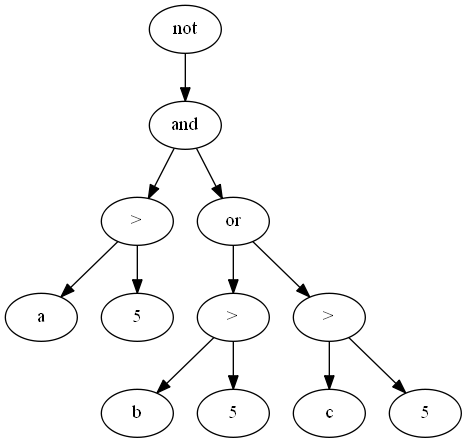
\includegraphics[scale=0.5]{Bilder/not_graph1.png} & 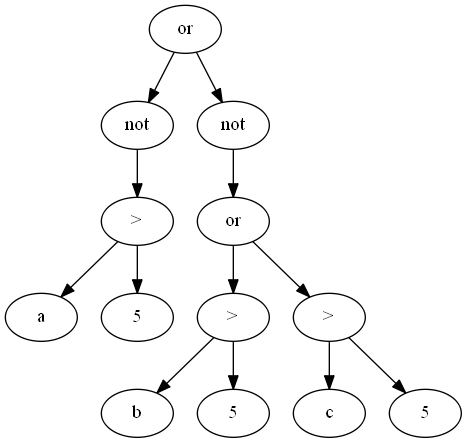
\includegraphics[scale=0.5]{Bilder/not_graph2.png}\\
\end{tabular}

\begin{tabular}{ll}
Umwandlung Teil 2: & Umwandlung Teil 3:\\
\verb|((a <= 5) or (not(b > 5) and not(c > 5)))| & \verb|((a <= 5) or ((b <= 5) and (c <= 5)))|\\
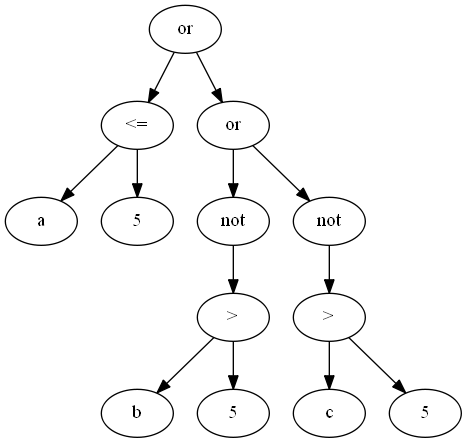
\includegraphics[scale=0.5]{Bilder/not_graph3.png} & 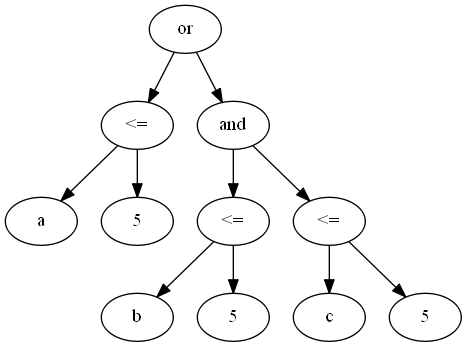
\includegraphics[scale=0.5]{Bilder/not_graph4.png}\\
\end{tabular}


\subsubsection{Anwenden des Distributivgesetzes}

Im letzten Schritt haben wir die Formel \verb|((a <= 5) or ((b <= 5) and (c <= 5)))| erhalten. Durch Anwenden des Distributivgesetzes können wir diese Formel im letzten Schritt umformen zu: \verb|((a <= 5) or (b <= 5)) and ((a <= 5) or (c <= 5))|

\subsection{Ersetzung von syntaktischen Varianten}

Um eine Anfrage zu standardisieren müssen wir den syntaktischen Zucker entfernen. Dies geschieht, indem man nur eine syntaktische Schreibweise anerkennt und alle anderen Schreibweisen in die zulässige umgewandelt. Zu erwähnen sind folgende Ersetzungen, die durchgeführt werden sollen um syntaktisch vielfältige, aber semantisch äquivalente Ausdrücke zu minimieren:

\begin{figure}[h]
\begin{tabular}{ccl}
\verb|A BETWEEN B AND C| & $\to$  & \verb|A >= B AND A <= C|\\
\verb|SELECT ALL| & $\to$ & \verb|SELECT|\\
\verb|ORDER BY VAR ASC| &  $\to$ & \verb|ORDER BY VAR|\\
\verb|A IN ('X', 'Y', 'Z')| & $\to$ & \verb|A = 'X' OR A = 'Y' OR A='Z'|\\
\verb|EXISTS (SELECT A,B,C ...)| & $\to$ & \verb|EXISTS (SELECT 1 ...)|\\
\end{tabular}
\caption{Entfernen von syntaktischen Varianten}
\end{figure}

\subsubsection*{Unteranfragen}

Es ist bekannt, dass sämtliche Typen von Unteranfragen eliminiert oder durch \verb|EXISTS|-Anfragen ersetzt werden können. Streng genommen handelt es sich hier zwar um mehr als nur eine syntaktische Variante, aber dennoch wollen wir das Ersetzen von Unteranfragen in diesem Abschnitt betrachten.
\subsubsection*{Ersetzen von ALL}

\verb|... SAL >= ALL(1000, LOW_SAL)|  wird zu:\\
\verb|... SAL >= 1000 AND SAL >= LOW_SAL|

\subsubsection*{Ersetzen von ANY/ SOME}

\begin{verbatim}
X.SAL >= ANY(SELECT Y.SAL FROM EMP Y 
             WHERE Y.JOB = 'CLERK')
\end{verbatim} zu
\begin{verbatim}
EXISTS(SELECT Y.SAL FROM EMP Y 
       WHERE Y.JOB = 'CLERK' 
       AND X.SAL >= Y.SAL)
\end{verbatim}

Befindet sich ein \verb|NOT| vor der Unteranfrage, so wird dieses nicht zur Unterabfrage ``durchgedrückt'' sondern bleibt davor.

\subsubsection{Ersetzen von IN}

Unter bestimmten Voraussetzungen kann jede IN-Unterabfrage in eine äquivalente EXISTS-Unteranfrage umgewandelt werden.

Wir wandeln IN-Unteranfragen wie die Folgende:

\begin{lstlisting}[mathescape]
$t_1$ IN (SELECT $t_2$
      FROM $R_1\ X_1$, ..., $R_n\ X_n$
      WHERE $\varphi$)
\end{lstlisting}

unter Voraussetzungen, die noch erläutert werden, um in:

\begin{lstlisting}[mathescape]
EXISTS (SELECT *
        FROM $R_1\ X_1$, ..., $R_n\ X_n$
        WHERE ($\varphi$) AND $t_1 = t_2$)
\end{lstlisting}

Folgende Voraussetzungen müssen erfüllt sein, damit diese Umwandlung angewendet werden kann:

\begin{itemize}
\item Alle Tupelvariablen, die in $t_1$ vorkommen, müssen sich unterscheiden von allen $X_i$. Erreicht wird dies ggf. durch Umbenennung der $X_i$, da diese nicht für die eigentliche (Ober)anfrage wichtig sind.
\item Wenn $t_1$ Attributreferenzen $A$ ohne Tupelvariable enthält, dann dürfen die $R_i$ kein Attribut $A$ haben. Erreicht wird dies, indem ggf. die Tupelvariable eingeführt wird.
\item Die Unteranfrage für $t_2$ darf keine Nullwerte liefern.
\end{itemize}

\subsubsection{Andere Unteranfragen}

Ungewöhnliche Unterabfragen, wie \mbox{z. B.} Unterabfragen unter \verb|FROM| werden hier nicht betrachtet. Im Allgemeinen werden solche Unterabfragen kaum gebraucht und machen die Anfrage meist nur viel komplexer als notwendig.

\subsubsection{JOINS}
Ein \verb|INNER JOIN| kann sowohl im \verb|FROM|-, als auch im \verb|WHERE|-Teil einer SQL-Anfrage formuliert werden. Damit Untersuchungen einheitlich geschehen können, formulieren wir solche JOINs im \verb|WHERE|-Teil der SQL-Anfrage.

\begin{figure}[h]
Eingabe:\\
\verb|SELECT * FROM foo f INNER JOIN bar b ON f.id=b.id|\\

Umwandlung:\\
\verb|SELECT * FROM foo f, bar b WHERE f.id=b.id|\\
\caption{Umwandlung von INNER-JOIN}
\end{figure}

Bei Anwendung dieser Ersetzungsregeln, soll dem Lernenden ein klares Feedback gegeben werden. Es soll verdeutlicht werden, dass eine korrekte Anfrage dennoch Mängel aufweist, da unnötige Formulierungen benutzt wurden.

Es ist hier bereits möglich Terme, die nur aus numerischen Konstanten bestehen, zu ersetzen durch das jeweilige Ergebnis. So könnten arithmetische Operationen bereits ausgeführt und Vergleiche, die nur aus numerischen Konstanten bestehen, durch entsprechende Wahrheitswerte ersetzt werden.

\subsection{JOIN-Eliminierung}

In einem weiteren Zwischenschritt möchten wir gern einige unnötige \verb|JOINS| eliminieren.

\subsubsection{OUTER JOIN}

Betrachten wir eine SQL-Anfrage mit einem \verb|OUTER JOIN|. Befinden sich im \verb|SELECT|-Teil keine Attribute der \verb|JOIN|-Tabelle, so ist der \verb|JOIN| unnötig, weil Daten von der \verb|JOIN|-Tabelle ohnehin nicht ausgegeben werden. Betrachten wir dazu folgendes Beispiel:

\begin{figure}[h]
\begin{lstlisting}[mathescape]
SELECT s.vorname, s.nachname 
FROM studenten s LEFT JOIN klausur k ON s.id = k.id 
WHERE k.wert <= 3
\end{lstlisting}
\caption{Unnötiger OUTER JOIN}
\label{fig:joinelem1}
\end{figure}

Im Beispiel in Abbildung \ref{fig:joinelem1} sollen alle Studenten ausgegeben werden, die in einer Klausur die Note drei oder besser bekommen haben. Da es sich hier um einen \verb|OUTER JOIN| handelt und wir nur Namen der Studenten ausgeben möchten, erhalten wir immer eine gesamte Liste der Studentennamen. Der Teil, der für den \verb|JOIN| interessant wäre, also Daten aus der Tabelle \verb|klausur k|, wird nicht ausgegeben. Damit wäre die folgende SQL-Anfrage mit der aus Abbildung \ref{fig:joinelem1} äquivalent.

\begin{figure}[h]
\begin{lstlisting}[mathescape]
SELECT s.vorname, s.nachname 
FROM studenten s 
\end{lstlisting}
\caption{Anfrage ohne JOIN}
\label{fig:joinelem2}
\end{figure}

Bei einem \verb|RIGHT JOIN| müsste man äquivalent überprüfen ob man Attribute im \verb|SELECT|-Teil hat, die in der ``linken'' Tabelle sind und genauso verfahren.

Möchte man tatsächlich nur die Studenten ausgeben, die eine drei oder besser geschrieben haben, müsste man einen \verb|INNER JOIN| verwenden.

\subsubsection{Transitiv-implizierte INNER JOINs}

Wenn nur Schlüsselattribute einer Tupelvariable X benutzt werden und diese mit \hyphenation{Fremd-schlüs-sel-at-tri-but-en} einer anderen Tupelvariable Y verglichen werden, dann ist X überflüssig.

In der Arbeit \cite{joinelem2} wird dazu ein Algorithmus angegeben, der im Wesentliche oben genannte, überflüssige Tupelvariablen entfernt. Wir wandeln diesen Algorithmus leicht ab, erhalten aber die Grundidee.

Im ersten Schritt erstellen wir transitiv-abgeschlossene Äquivalenzklassen der Attribute, die im \verb|WHERE|-Teil vorkommen. Haben wir also $X.A=Y.B$ und $Y.B=Z.C$, so befinden sich alle drei Attribute in einer Äquivalenzklasse: $\{X.A,Y.B,Z.C\}$. Eine Äquivalenzklasse enthält nur Tupelvariablen und ist transitiv abgeschlossen über dem Operator $=$.
Dabei bemerken wir, dass Äquivalenzklassen der Mächtigkeit 1 einfache Vergleiche wie \verb|X.A Operator Konstante| sind. Klassen der Mächtigkeit 2 sind einfache, nicht transitive JOINs und Klassen der Mächtigkeit größer als 2 sind offensichtlich mehrfache, transitive JOINs.

Beispiel:
\begin{lstlisting}[mathescape]
SELECT t1.x 
FROM   test1 t1, test2 t2, test3 t3
WHERE  t1.x = t2.y
AND    t1.x = t3.z
AND    t1.y = t2.z
AND    t1.z > 3;
\end{lstlisting}

Bei diesem Beispiel erhalten wir die Äquivalenzklasse \verb|{t1.x, t2.y, t3.z}| sowie die Klassen \verb|{t1.y,t2.z}| und \verb|{t1.z}|.

Im nächsten Schritt gehen wir jede Äquivalenzklasse durch, die mindestens drei Einträge haben. Für jeden Eintrag $e\in\mathit{Aequivalenzklasse}$ mit $e=T.A$ überprüfen wir, ob es andere Äquivalenzklassen gibt, die nicht aus einem transitiven \verb|JOIN| entstanden sind (also weniger als drei Einträge haben) und die ein Attribut der Tabelle $T$ enthalten. Ist dies nicht der Fall und die Tabelle $T$ kommt nicht im \verb|SELECT|-Teil vor, dann ist das Attribut $A$ in dem Vergleich, der durch die Äquivalenzklasse repräsentiert wird, unnötig und kann samt zugehöriger Bedingung im \verb|WHERE|-Teil gestrichen werden. Hat die Äquivalenzklasse jetzt weniger als drei Einträge dann wird die Arbeit an dieser Klasse abgebrochen.

Im letzten Schritt müssen wir noch überprüfen, ob es Tupelvariablen im \verb|FROM|-Teil gibt, die aber nun nicht mehr im \verb|WHERE|-Teil auftauchen. Ist dies der Fall, dann streichen wir diese aus dem \verb|FROM|-Teil.

NULL bearbeiten

Beispiel:
\begin{lstlisting}[mathescape]
SELECT ps.partkey, avg(ps.supplycost)
FROM   supplier s, partsupp ps, customer c, orders o
WHERE  s.suppkey = ps.suppkey 
AND    s.suppkey = c.custkey
AND    c.custkey = o_custkey
AND    o_totalprice >= 100;
\end{lstlisting}

Zunächst erzeugen wir alle Äquivalenzklassen:
\begin{lstlisting}[mathescape]
Klassen = 
$\{ \{$s.suppkey, ps.suppkey, c.custkey,o.custkey $\}, \{$o.totalprice$\} \}$
\end{lstlisting}

Die zweite Menge interessiert uns nicht, da sie nicht mehr als zwei Elemente enthält. Wir betrachten daher nur die erste Menge. Wir untersuchen nun jedes einzelne Element auf seine Gültigkeit. \verb|s.suppkey| kommt in keiner anderen Äquivalenzklasse vor und die Tabelle \verb|supplier s| erscheint nicht im \verb|SELECT|-Teil, daher streichen wir \verb|s.suppkey|. Das nächste Attribut \verb|ps.suppkey| kann nicht gestrichen werden, da die Tabelle \verb|partsupp ps| im \verb|SELECT|-Teil erscheint. \verb|c.custkey| kann wiederum gestrichen werden, da es wieder nicht in einer anderen Äquivalenklasse auftaucht und die Tabelle \verb|customer c| nicht im \verb|SELECT|-Teil auftaucht. Dahingegen ist \verb|o.custkey| nicht zu streichen, da die Tabelle \verb|orders o| in einer Äquivalenzklasse auftaucht, welche nicht zu einem \verb|JOIN| gehört (weil sie weniger als drei Elemente beinhaltet). Nun können wir auch die Tabellen \verb|supplier s| und \verb|customer c| streichen, da keine Bedingung mehr Attribute aus diesen Tabellen enthält.

Daher erhalten wir nun die folgende, optimierte Anfrage:
\begin{lstlisting}[mathescape]
SELECT ps.partkey, avg(ps.supplycost)
FROM   partsupp ps, orders o
WHERE  o.custkey = ps.suppkey 
AND    o.totalprice >= 100;
\end{lstlisting}

PSEUDOCODE:

\begin{lstlisting}[mathescape]
Alle Attribute im WHERE-Teil in Aequivalenklassen $E_i$ packen.
foreach $e\in E_i$ mit $\vert e\vert \ge 3$ do
  foreach $t.a\in e$ do
    if $\vert e\vert \ge 3$ and $t \notin $SELECT and 
    $\nexists b\in E_i$ mit $\vert b\vert < 3$ und b=t.*
      e = e - {t.a}
    end
  done
done

Streiche unnoetige Tabellen aus FROM-Teil 
\end{lstlisting}

\subsection{Operatorenvielfalt}

Im folgenden Abschnitt soll geklärt werden wie mit verschiedenen Schreibweisen von ein- und demselben Ausdruck umgegangen werden soll. Betrachtet man sich \mbox{z. B.} \verb|A > 5| ist dieser Ausdruck äquivalent mit \verb|5 < A|. Wenn wir wissen, dass \verb|A| ein ganzzahlige Variable ist, dann sind auch folgende Äquivalenzen wahr: \verb|A >= 6| sowie \verb|6 <= A|. Wir betrachten nun zwei verschiedene Ansätze um mit diesem Problem umzugehen. Der erste Ansatz beschäftigt sich damit, alle implizierten Schreibweisen mit in die Formel aufzunehmen. Damit stellt man sicher, dass sich alle korrekten Schreibweisen einer Formel in der Anfrage befinden. Der zweite Ansatz beschäftigt sich damit, nur bestimmte Schreibweisen zuzulassen und alle anderen durch die zulässigen zu ersetzen.

Hinweis: Diesem Schritt geht eine Teilsortierung vor. Diese wird ebenfalls im Abschnitt >>Sortierung<< erwähnt. 

\subsubsection{Teilsortierung}

Wir betrachten Ausdrücke mit den Operatoren $\{>,<,\leq,\geq,=,+,\cdot\}$. Da es sich hier jeweils um binäre Operatoren handelt, sprechen wir, im Sinne der Anordnung, im Folgenden von einem linken und einem rechten Operanden. Ist einer der Operanden eine Variable, so wird diese links angeordnet. Sind beide Operanden Variablen, so werden sie lexikographisch-sortiert angeordnet. Operanden, die selbst wieder zusammengesetzte Ausdrücke sind, stehen rechts. Sind beide Operanden zusammengesetzte Ausdrücke, so steht der komplexere rechts und der weniger komplexe links. Ein Ausdruck $A$ ist komplexer als ein Ausdruck $B$, wenn der zugehörige Operatorbaum von $A$ tiefer ist als der Operatorbaum von $B$. Sind beide Ausdrücke gleich komplex, so wird die symmetrische Variante mit hinzugenommen. Wenn wir Operanden umsortieren bei denen der Operator $\in \{>,<,\leq,\geq\}$ ist, dann muss der jeweilige Operator auch umgedreht werden. Bei den restlichen Operatoren ist dies nicht der Fall, da diese symmetrisch sind.

\subsubsection{Hinzufügen implizierter Formeln}

Trifft man im Parserbaum auf eine Formel, zu der es mehrere äquivalente Formeln gibt, so ist ein Ansatz alle diese äquivalenten Formeln konjunktiv zu verknüpfen und mit in den Parserbaum aufzunehmen. Treffen wir also zum Beispiel auf folgenden Ausdruck: \begin{verbatim}SELECT * FROM testtable WHERE A = B - C\end{verbatim}, , so müssen wir auch alle äquivalenten Formeln mit aufnehmen. Daraus wird dann also der Ausdruck: \begin{verbatim}...WHERE A = B - C AND B = A + C AND C = B - A\end{verbatim}

Wie man bereits sieht, sind die hinzugefügten Formeln redundant und tragen nicht effizient zur Beschleunigung der Anfrage bei. Es soll hier lediglich sichergestellt werden, dass alle möglichen äquivalenten Formeln auftreten, da wir nicht wissen, was der Student für einen Repräsentanten der Formeln wählen wird. Weiterhin muss bemerkt werden, dass dadurch die gesamte SQL-Anfrage enorm aufgebläht wird. Es ist daher unbedingt wichtig, die Originalanfrage zu speichern. Weiterhin muss das Programm eine Verbindung zwischen den Formeln der Originalanfrage und den Formeln der veränderten, aufgeblähten Anfrage herstellen. Dem Lernenden soll in einem Feedback nur Fehler in der Originalanfrage aufgezeigt werden. Da intern aber mit der aufgeblähten Anfrage gearbeitet wird, muss beim Auftreten eines Fehlers oder Hinweises nachgeschlagen werden, von welchem Teil der Originalanfrage der Teil entstammt, der jetzt den Fehler auslöst.

Im Folgenden listen wir Mengen $M_i$ von Ausdrücken. Finden wir in der zu bearbeitenden SQL-Anfrage eine Formel $f$, die auf einen Ausdruck $a\in M_i$ passt, dann verknüpfen wir alle Ausdrücke $\{b : b\in M_i \wedge b \neq a\}$ konjunktiv mit $f$. Dabei sind alle Variablennamen $A,B,C$ keine (komplexen) Ausdrücke. Es handelt sich also jeweils um Blattknoten im Parserbaum. Ferner bezeichnen wir $X,Y$ als numerische Konstanten.\\

\begin{tabular}{ll}
$M_1$ & $\{\ A=B-C\ ,\ C=B-A\ ,\ B=A+C\ \}$\\
$M_2$ & $\{\ A=B\cdot C\ ,\ C=A / B\ ,\ B=A / C\ \}$\\
$M_3$ & $\{\ A>B-C\ ,\ C>B-A\ ,\ B<A+C\ \}$\\
$M_4$ & $\{\ A<B-C\ ,\ C<B-A\ ,\ B>A+C\ \}$\\
$M_5$ & $\{\ A>B, B<A \}$\\
$M_6$ & $\{\ A\geq B, B\leq A \}$\\
$M_7$ & $\{\ A>X, A\geq X+\mathit{adjust}(A) \}$\\
$M_8$ & $\{\ A<X, A\leq X-\mathit{adjust}(A) \}$\\

\end{tabular}

Beim Vergleich mit $>$ und $<$ ist es wichtig zu wissen, wie viel Nachkommastellen die numerischen Variablen $A$ und $B$ besitzen. Es sei $\mathit{places}(A)$ die Anzahl der Nachkommastellen der Zahl $A$. Dann bezeichnen wir mit $\mathit{adjust}(A) = 1 / (10^{\mathit{places}(A)})$, einen angepassten Wert, der sich nach der Stelligkeit der Variable A richtet.

Betrachten wir als Beispiel ein Attribut \verb|salery|, welches als \verb|NUMERIC(4,2)| definiert ist. Wir wissen also, dass \verb|salery| zwei Nachkommastellen hat. Betrachten wir nun die Aussage \verb|salery >= 5|.
Wir haben auf einer Seite eine Variable (\verb|salery|) und auf der anderen Seite eine numerische Konstante (\verb|5|). Dieses Muster passt also auf $M_7$ und auf $M_6$. In $M_7$ heißt es $A\geq X+\mathit{adjust}(A)$. Bezogen auf unser Beispiel ist \verb|A=salery| und \verb|x+adjust(salery)=5|. Wir berechnen also: 
$$\mathit{adjust}(\mathit{salery}) = 1 / (10^{2}) = 1/100 = 0,01$$
Wir erhalten also \verb|x=4,99|, weil \verb|x+0,01=5|. Somit ergänzen wir unsere Ausgangsformel \verb|salery >= 5| konjunktiv mit \verb|salery > 4,99|. Weiterhin muss jetzt wegen $M_6$ \verb|5 <= salery| und wegen $M_5$ \verb|4,99 < salery| hinzugefügt werden.

Finden wir Ausdrücke mit $>,<,\leq,\geq$, welche als Argumente Variablen oder Konstanten haben, so unterscheiden wir also grundsätzlich drei Fälle.

Fall 1 $(M_5,M_6)$: Beide Operanden sind Variablen oder Konstanten. In diesem Fall ergänzen wir nur den jeweils symmetrischen Operator. Da beide Operanden Variablen sind, macht es keinen Sinn jeweils $\leq,\geq$ oder $<,>$ zu ersetzen.

Fall 2 $(M_7,M_8)$: Einer der beiden Operanden ist eine numerische Konstante und der andere ist eine Variable. In diesem Fall fügen wir alle implizierten Gleichungen hinzu, also insbesondere die Operatoren $\leq,\geq,<,>$. Zu beachten ist hier, dass nicht nur Gleichungen der Form $A>X$ dazu führen, dass alle Ausdrücke von $M_7$ hinzugefügt werden. Auch wenn eine Gleichung der Form $Var1\geq 5.2$ auftaucht, werden Ersetzungen durchgeführt. Diese Gleichung passt auf das Muster $A\geq X+\mathit{adjust}(A)$. Angenommen $Var1$ hat maximal eine Nachkommastelle, so würden dann folgende Gleichungen impliziert werden: $\{\ Var1>5.1\ ,\ 5.1<Var1\ ,\ 5.2 \leq Var1\ \}$.

Fall 3: Beide Operanden sind numerische Konstanten. In dem Fall wird die logische Aussage ausgewertet und durch ihren Wahrheitswert ersetzt [0,1].

Sind durch die hinzugefügten Terme nun arithmetische Ausdrücke entstanden, die nur noch numerische Konstanten enthalten, so werden diese Ausdrücke ausgewertet.

Dieser Teilschritt erfordert weiterhin eine Sortierung der einzelnen Terme.

\subsubsection{Beschränkung der Operatorenvielfalt}

Ein weiterer Ansatz das Problem der äquivalenten Formeln anzugehen ist es, bestimmte Operatoren zu >>verbieten<<. Das soll bedeuten, wir definieren verbotene Operatoren, welche am Ende der Umwandlungen nicht mehr in der SQL-Anfrage vorkommen dürfen. Dies wird erreicht, indem wir jeden verbotenen Operator umwandeln in einen nicht-verbotenen Operator. Das Prinzip ähnelt dem eben Vorgestellten. Wir betrachten wieder die Mengen $M_i$. Des Weiteren hat jede Menge $M_i$ einen Repräsentanten $r(M_i)$. Finden wir nun in der zu bearbeitenden Anfrage eine Formel $f$, die auf eine der Ausdrücke $a\in M_i$ passt, so ersetzen wir $f$ mit $r(M_i)$. Folgende Tabelle soll die Mengen und deren Repräsentanten beschreiben.

Im folgenden sind alle Variablennamen $A,B,C$ keine (komplexe) Ausrücke. Es handelt sich also jeweils um Blattknoten im Parserbaum. Ferner bezeichnen wir $X,Y$ als numerische Konstanten.\\

\begin{tabular}{lll}
$i$ & $M_i$ & $r(M_i)$ \\
$1$ & $\{\ A=B-C\ ,\ C=B-A\ ,\ B=A+C\ \}$ & $B=A+C$\\
$2$ & $\{\ A=B\cdot C\ ,\ C=A / B\ ,\ B=A / C\ \}$ & $A=B\cdot C$\\
$4$ & $\{\ A>B-C\ ,\ C>B-A\ ,\ B<A+C\ \}$ & $A>B-C$ \\
$5$ & $\{\ A<B-C\ ,\ C<B-A\ ,\ B>A+C\ \}$ & $A<B-C$\\
$6$ & $\{\ A>B, B<A \}$ & $A>B$\\
$7$ & $\{\ A\geq B, B\leq A \}$ & $A\geq B$\\
$8$ & $\{\ A>X\ ,\ X<A,A\geq X+\mathit{adjust}(X)\ ,\ X\leq A - \mathit{adjust}(X)\ \}$ & $A>X$\\
\end{tabular}

Im Folgenden soll ein Beispiel die Prozedur verdeutlichen.\\

Es sei unsere Ausgangsanfrage: \begin{verbatim}SELECT * FROM testtable WHERE X = 6 - Y\end{verbatim}

Die Formel $X=6-Y$ finden wir in $M_1$ in Form von $A=B-C$. Wir ersetzen nun also $X=6-Y$ mit dem Repräsentanten von $M_1$, und wir bekommen: \begin{verbatim}SELECT * FROM testtable WHERE 6 = X + Y\end{verbatim}

\subsubsection{Diskussion der beiden Ansätze}

Ein wesentlicher Punkt beim Vergleich beider Ansätze ist der Aufwand bzw. die Laufzeit. 

Betrachten wir zunächst den Ansatz des Hinzufügens von implizierten Formeln. Wir müssen in einer Tiefensuche jede Formel betrachten und mit allen Mengen $M_i$ abarbeiten. Finden wir in einer Menge ein Muster wieder, so wird unsere Formel künstlich aufgebläht. Wir haben also für das Suchen eine maximale Laufzeit von $\mathcal{O}(\mathit{\vert Formeln\vert \cdot max\{i : M_i\}})$. Das Einfügen der Formeln geschieht in konstanter Zeit $\mathcal{O}(1)$, da wir immer eine konstante Anzahl an Formeln ergänzen.

Beim anderen Ansatz werden bestimmte Operatoren verboten. Wir realisieren dieses Verbot wieder über eine Suche. Es muss auch hier jede Formel auf ein Muster in $M_i$ untersucht werden. Wir benötigen für das Suchen in diesem Ansatz also genau so viel Zeit, wie im ersten Ansatz. Auch das Ersetzen der Formeln hat keine Zeitersparnis gegenüber einem Hinzufügen von weiteren Formeln. Es muss bemerkt werden, dass in diesem Fall die Originalformel nicht weiter aufgebläht wird.

Da sich die Laufzeiten der beiden Varianten nicht unterscheiden, müssen andere Kriterien zum Vergleich herangezogen werden. Wichtig für Software ist nicht ausschließlich die Laufzeit, sondern auch die Wartbarkeit. Besonders bei Projekten, die im Rahmen einer Masterarbeit entstehen, ist es wahrscheinlich, dass der Autor sich später nicht mehr um das Projekt kümmern kann. Daher sollte man sich bei den hier vorliegenden Ansätzen fragen, welcher leichter wartbar und erweiterbar ist.

Muss das Programm erweitert werden und wir möchten den Ansatz des Hinzufügen implizierter Gleichungen verwenden, so muss lediglich eine weitere Menge $M_k$ erstellt werden. Der Algorithmus sucht automatisch, dann auch in dieser neuen Menge nach Mustern und würde alle anderen Elemente dieser Menge konjunktiv-verknüpft zur Formel hinzufügen. 

Bei der Verwendung von eingeschränkten Operatoren gestaltet sich dieser Ansatz bereits als schwierig. Hier muss man nicht nur die neue Menge $M_k$ angeben, sondern sich auch Gedanken machen, was ein geeigneter Repräsentant dieser Menge ist. Unter Umständen kann das Auswählen eines ungünstigen Repräsentanten zu unerwarteten Problemen, wie dem Verkomplizieren der Anfrage, führen.

Es bietet sich aus diesen Umständen eher an, das Hinzufügen von implizierten Gleichungen zu verwenden.

\subsection{Sortierung}

Im aktuell betrachteten Ansatz möchten wir zwei Anfragen dadurch vergleichen, dass wir sowohl die Musterlösung, als auch die Studentenlösung einer Standardisierung unterziehen. Ein ganz wesentlicher Aspekt dabei ist, die Art der Sortierung. Sind die ZQL-Parserbäume isomorph zueinander, dann lässt sich das leicht zeigen, in dem man beide nach gleichartigen Kriterien sortiert und dann einen direkten Abgleich vornimmt.

Dabei unterscheiden wir zwei Arten von Sortierung: Hat ein Operator als Operanden nur Ausdrücke und keine Konstanten oder Variablen dann sortieren wir die Kindknoten, welche jeweils wieder eigene Terme bilden.

Hat ein Operator als Operand mindestens eine Konstante oder Variable, so sortieren wir das innere dieses Terms.

\subsubsection{Sortierung im Inneren der Terme}

Hat ein Operator \textit{OP1} als Kindknoten mindestens ein Blatt, dann werden die Kindknoten so sortiert, dass zunächst die Blattknoten (lexikographisch) und erst dann die Teilbäume erscheinen. Möglich wird dies, weil die Tabellen-Aliase in einem vorherigen Schritt bereits automatisch sortiert und benannt wurden. Bei symmetrischen Operatoren wie $=,  \textit{AND}, \textit{OR}$ können die Kindknoten einfach umgehangen/ umsortiert werden. Bei Operatoren wie $\le,\ge$ ist es notwendig den Operator \textit{OP1} umzudrehen. Weil aber die Sortierung außerhalb von Termen auf den Operatoren basiert, ist es notwendig, die Sortierung im Inneren der Terme zuerst durchzuführen.

Dieser Schritt wurde bereits als Vorbereitung der Schritte >>Hinzufügen von implizierten Formeln<< und >>Operatorbeschränkung<< durchgeführt. 

\subsubsection{Sortierung von Termen}

Hat ein Operator \textit{OP1} als Kindknoten nur weitere Operatoren \textit{OP2,OP3}, dann muss anhand dieser Operatoren die Reihenfolge im Baum festegelegt werden. Dies geschieht, indem wir uns einfach eine Reihenfolge der Operatoren ausdenken. Wir überlegen uns folgende Ordnung $order:\textit{Relation}\to\mathbb{N}$, in der eine Relation $r$ vor einer Relation $s$ im standardisierten Parserbaum erscheint, wenn $order(r) < order(s)$.

$order:$\\

\begin{tabular}{|llllllll|}
\hline
$r\in \textit{Relation}$ & $\le$ & $\ge$ & $>$ & $<$ & $=$ & IS NULL & IS NOT NULL  \\
$\textit{order}(r)$ & 1 & 2 & 3 & 4 & 5 & 6 & 7\\ 
\hline
\end{tabular}\\

Es sei $\textit{RT}(\textit{OP})$ der Teilbaum des SQL-Ausdruckes mit der Wurzel \textit{OP}. Wir bezeichnen mit $\textit{depth}(\textit{RT}(\textit{OP}))$ die Tiefe des Baumes $\textit{RT}(\textit{OP})$. Es seien $\textit{child}(\textit{OP}) = \{v_1,v_2,...,v_i,...,v_n\}$ die Kindknoten von $\textit{OP}$. Die korrespondierenden Teilbäume $\textit{RT}(v_1),\textit{RT}(v_2),...,\textit{RT}(v_i),...,\textit{RT}(v_n)$ sollen nun wie folgt angeordnet werden: Der Teilbaum $\textit{RT}(v_x)$ erscheint (bei einer fiktiven BFS) vor dem Teilbaum $\textit{RT}(v_y)$ genau dann, wenn $\textit{depth}(\textit{RT}(v_x)) <  \textit{depth}(\textit{RT}(v_y))$. Die Teilbäume werden also der Tiefe nach aufsteigend angeordnet. 

Wie bereits im Abschnitt >>Teilsortierung<< angedeutet, werden Teilbäume mit gleicher Tiefe nicht sortiert. In diesem Fall erzeugen wir einen Alternativbaum, indem wir die zwei betreffenden Teilbäume vertauschen. Mit diesem Alternativbaum wird dann, parallel zum bisherigen Baum, weiter verarbeitet. Am Ende muss die Musterlösung auch gegen alle Alternativlösungen geprüft werden.

Eine weitere Alternative zur Behandlung von Teilbäumen mit gleicher Tiefe, ist die Sortierung Anhand der Blattknoten. Dazu sammeln wir in einer Tiefensuche die Werte der Blattknoten und hängen sie in einem String zusammen. Es seien also die Knoten $V_{DFS} = \{v_1,v_2,...,v_k\}$ die Knoten, die in einer Tiefensuche eines (Teil)baumes entstehen. Wir bezeichnen den Blattknotenstring eines gewurzelten Baumes, mit dem Operator $O$ als Wurzel, mit: $$\mathit{leaf\_string}(RT(O)) = \mathit{val}(v_1) \oplus \mathit{val}(v_2) \oplus ... \mathit{val}(v_k)$$

Dabei bezeichnen wir mit $\mathit{val}(v_k)$, den Wert eines Blattknotens.

$$
val(v)=\begin{cases}
  \text{Variablenname},  & \text{wenn }v\text{ Variable,}\\
  \text{Wert}, & \text{wenn }v\text{ eine Konstante.}
\end{cases}
$$

Aus den Teilbäumen mit gleicher Tiefe, werden solche Strings erzeugt und diese dann verglichen.
Ist $\mathit{leaf\_string}(RT(O_1)) <  \mathit{leaf\_string}(RT(O_2))$, so wird der Teilbaum $RT(O_1)$ als erstes Kind im Baum auftauchen.

\begin{figure}[h]
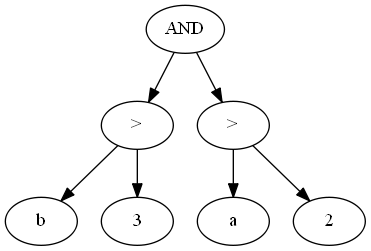
\includegraphics[scale=0.5]{Bilder/same_depth1.png}         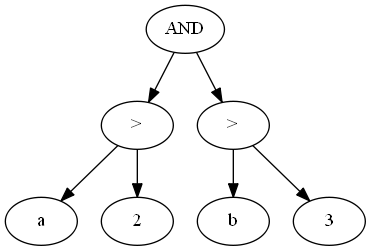
\includegraphics[scale=0.5]{Bilder/same_depth2.png}
\caption{Beispiel von Bäumen mit gleicher Tiefe}
\label{fig:bsp1}
\end{figure}

Wir sehen in Abbildung \ref{fig:bsp1}, auf der linken Seite, zwei Teilbäume mit Wurzelknoten $>$. Wir bezeichen den linken Teilbaum mit $RT(>_l)$ und den rechten mit $RT(>_r)$. Somit ergeben sich $\mathit{leaf\_string}(RT(>_1)) = \mathit{val}(b) \oplus  \mathit{val}(3) = 'b3'$ und 
$\mathit{leaf\_string}(RT(>_2)) = \mathit{val}(b) \oplus  \mathit{val}(3) = 'a2'$. Wegen $\mathit{a2} < \mathit{b3}$ tauschen die Teilbäume ihre Position und ergeben das rechte Bild in Abbildung \ref{fig:bsp1}. Da wir diesem Schritt die Tupelvariablen bereits durch automatische Variablennamen vereinheitlicht haben, kann der gesamte Name des Attributs samt Präfix der Tupelvariable als $\mathit{val()}$ angesehen werden.

\subsection{Abschluss}

Wir fassen die einzelnen Schritte noch einmal kurz zusammen: Zunächst haben wir den \verb|FROM|-Teil der Anfrage vereinheitlicht, indem wir einheitliche Tupelvariablen erzeugt haben, nachdem alle Tabellen im \verb|FROM|-Teil lexikographisch sortiert wurden. Alle neu erzeugten Variablennamen wurden im Rest der Anfrage korrekt eingesetzt bzw. ersetzt. Danach haben wir den \verb|WHERE|-Teil bearbeitet. Wir haben zunächst unnötige Klammern entfernt und die Formeln in die KNF überführt. Danach haben wir einfache syntatkische Varianten ersetzt um eine einheitlichere Darstellung zu erhalten. Dazu gehörte es auch Unteranfragen aufzulösen oder, wenn nicht möglich, in eine \verb|EXISTS|-Unteranfrage zu überführen. Danach haben wir innere Verbunde (JOINs), die im \verb|FROM|-Teil formuliert wurden, in den \verb|WHERE|-Teil überführt, um anschließend unnötige äußere Verbunde und unnötige transitive, innere Verbunde  zu eliminieren. Eine der letzten Schritte war das Behandeln der Vielfalt der Operatoren. Dem ging zunächst eine Teilsortierung des Parserbaumes voraus. Mit einer der beiden vorgestellten Methoden haben wir nun alle implizierten Formeln hinzugefügt, oder die Operatoren gemäß ihrer Repräsentanten beschränkt. Schlussendlich haben wir den gesamten \verb|WHERE|-Teil sortiert, um eine Vereinheitlichung zu erreichen.

\section{Anpassung durch elementare Transformationen}

Der nun vorgestellte Ansatz stellt eine Alternative zur >>Anpassung durch Standardisierung<< dar. Beide Ansätze haben ähnliche Ideen, sind jedoch in ihrer Umsetzung verschieden. Beim Ansatz der Standardisierung haben wir zunächst eine SQL-Anfrage genommen und standardisiert. Dies geschah völlig unabhängig zu der zu vergleichenden, zweiten SQL-Anfrage. Es wurden gewisse allgemeine Regeln aufgestellt und nach diesen wurde jede SQL-Anfrage behandelt und angepasst. Der eigentliche Vergleich geschah dann aufgrund eines Vergleichs der standardisierten Anfragen und dem Vergleich von Metadaten (Anzahl Joins, Anzahl atomarer Formeln, etc.). Ein Nachteil von diesem Ansatz ist, dass wir für jedes mögliche Konstrukt in der SQL-Anfrage auch Regeln im System haben, damit wir jene Konstrukte auch anpassen und standardisieren können. Außerdem findet der Vergleich erst im allerletzten Schritt statt.

Die >>Anpassung durch elementare Transformationen<< stellt einen intuitiven Ansatz vor. Wir versuchen hier per Backtracking konkret eine Lösung der anderen anzugleichen. Damit haben wir einen konkreten Unterschied zum bisherigen Ansatz. Wir vergleichen die Lösung direkt und umgehen die Vorverarbeitungen. Im Wesentlichen geben wir also ganz allgemeine Regeln an und in jedem Schritt versuchen wir durch Anwendung dieser Regeln die SQL-Anfrage so anzupassen, dass sie auf unsere zu vergleichende Anfrage passt.

\subsection{Backtracking}

[Dieser Abschnitt ist experimentell]

Für das Backtracking an sich bietet sich die Programmiersprache PROLOG an. Das liegt daran, dass unsere allgemeine Regeln einfach formuliert werden können und bereits den Großteil des Programms stellen. Außerdem benutzt PROLOG die SLD-Resolution, um logische Anfragen auswerten zu können und das ist bereits ein Backtracking. Da wir in unserer Arbeit allerdings die Programmiersprache JAVA gewählt haben, können wir nicht auf PROLOG zurückgreifen. Viel mehr müssen wir das Backtracking selbst implementieren. 

Wir operieren weiterhin auf Parserbäumen, die so entstehen wie im Abschnitt >>Funktionsweise des Parsers<< erklärt wird. Es seien unsere zwei zu vergleichenden SQL-Anfragen mit \textit{Query1} und \textit{Query2} gegeben. Die dazugehörenden Parserbäume bezeichnen wir mit \textit{RT(Query1)} und \textit{RT(Query2)}. Wir versuchen im Folgenden \textit{Query1} an \textit{Query2} anzupassen.

Um nicht zu viele Regeln definieren zu müssen, werden wir Teile der Vorverarbeitung des ersten Ansatzes wieder verwenden. Wir formen beide Anfragen zunächst in die konjunktive Normalform um. Danach haben wir im Wesentlichen die folgenden, unterschiedlichen Fälle:

Zum einen haben wir kommutative Operatoren wie \verb|{+,*,AND,OR,=}|. Möchten wir zwei (Teil-)Bäume vergleichen, die einen solchen Operator als Wurzelknoten haben, so müssen wir uns im klaren sein, dass der gesuchte Operand an beliebiger Stelle auftauchen kann. Wir werden einen solchen Vergleich so angehen, dass wir uns den ersten Operanden aus Teilbaum 1 nehmen. Ist dieser Operand ein Ausdruck mit Operator $o_1$, dann suchen wir im zweiten Teilbaum nach einem Operanden, welcher auch ein Ausdruck ist mit Operator $o_2$ mit $o_1=o_2$. Ist dies gelungen, so wird verglichen, ob die Teilbäume mit der Wurzel $o_1$ und $o_2$ gleich sind. Dies geschieht dann rekursiv. Ist dies erfolgreich, so streichen wir aus den Ursprungsbäumen die Teilbäume mit Wurzel $o_1$ und $o_2$ und fahren mit dem nächsten Operanden aus dem ersten Teilbaum fort.

Operatoren, die nicht kommutativ sind, sind meistens Vergleichsoperatoren wie \verb|<=, < , > ,>=|. Haben wir zwei Teilbäume mit einem solchen Operator, so ist der Vergleich sehr einfach, denn die jeweiligen Teilbäume unter den Operatoren müssen absolut identisch sein. Dies wird wieder mittels Rekursion geprüft.

Haben wir im ersten Baum einen Vergleichsoperator ausgewählt und können diesen im zweiten Baum nicht finden, so müssen wir auch nach dem umgedrehten Operator in Baum 2 suchen. Finden wir einen solchen, dann vergleichen wir die zugehörigen zwei Teilbäume weiter rekursiv. Zu beachten ist dabei, dass sich die Operandenreihenfolge vom ersten Teilbaum auch umdreht.

\section{Weitere Betrachtungen}

Unabhängig von den bereits vorgestellten Ansätzen der >>Standardisierung<< und der >>Anpassung durch elementare Transformationen<< gibt es einige Umwandlungen, die entweder davor oder danach geschehen sollten. Diese Umwandlungen sollen dazu dienen dem Studenten ein Feedback zu geben. Das bedeutet, dass die Anfrage des Studenten richtig sein kann, allerdings unnötige oder unschöne Konstrukte enthält, welche die Anfrage unnötig kompliziert oder komplex machen.

Folgende verschiedene Komplexitätseinstufungen sollen eingeführt werden und auf jede Studentenanfrage angewendet werden.

\subsection{Anzahl atomarer Formeln}

Die Studentenanfrage enthält vor der Transformation durch unser Programm mehr atomare Formeln als die Musterlösung, so wurden offensichtlich unnötige Formeln oder doppelte Formeln aufgeschrieben. Stellt unser Programm fest, dass beide Lösungen dennoch gleich sind, so muss dem Studenten mitgeteilt werden, dass er redundante Formeln eingebaut hat, welche die Lösung unnötig verkomplizieren. 

\subsection{Anzahl der Operatorkompressionen}

Wie im vorherigen Abschnitt bereits erklärt ist der ZQL-Parserbaum nicht binär. Dadurch kann es durch zu vorsichtige Klammersetzung passieren, dass ein Teilbaum mit zwei Ebenen entsteht, obwohl nur ein Operator beteiligt ist. Erklärt ist dies im Abschnitt >>Funktionsweise des Parsers<<. Die dort vorgestellte Operatorkompression ist ein Verfahren um unnötige Klammerungen zu entfernen. Ist die Gleichheit der Lösung des Studenten mit der Musterlösung durch unser Programm gezeigt, aber die Studentenlösung musste mehr Operatorkompressionen durchführen, so hat der Student unnötige Klammern gesetzt, welche die Lösung wiederum unnötig verkomplizieren. Dies muss ihm durch unser Programm mitgeteilt werden.

\subsection{unnötiges DISTINCT}

Eine interessante Frage ist, ob ein \verb|DISTINCT| wirklich notwendig ist. Dies ist natürlich wichtig für den Vergleich zweier SQL-Anfragen. In \cite{brass2} wurde im Rahmen des SQLLint-Projektes bereits in dem Prototypen ein Checker eingebaut, der prüft ob \verb|DISTINCT| wirklich notwendig ist. Aber auch im Rahmen dieser Arbeit ist es notwendig zu wissen, ob das \verb|DISTINCT| notwendig ist. 

Auf den ersten Blick reicht es aus zu prüfen, ob die Musterlösung ein \verb|DISTINCT| enthält. Ist dies der Fall, so muss die Lösung des Lernenden das offensichtlich auch enthalten. Allerdings setzt dieser Denkansatz voraus, dass die eingetragene Musterlösung stets perfekt ist. Um Fehler vorzubeugen ist es besser, alle Anfragen auf unnötige \verb|DISTINCT| zu prüfen. So kann dem Korrektor beim Eintragen der Musterlösung bereits angezeigt werden, dass sein angegebenes \verb|DISTINCT| unnötig ist oder ob ein \verb|DISTINCT| notwendig wäre um Duplikate zu eliminieren. Auch wenn man sich weg bewegt vom Modell der Musterlösung und dem Vergleich mit dem Lernenden, ist dieser Check durchaus wichtig. Im Folgenden stellen wir daher einen Algorithmus vor, der erkennt ob die Lösung Duplikate enthalten kann oder nicht.

\subsection{Algorithmus aus \cite{sql1folien}}

Es sei unsere SQL-Anfrage der Form:

\begin{lstlisting}[mathescape]
SELECT $t_1$, ..., $t_k$
FROM $R_1\ X_1$, ..., $R_n\ X_n$
WHERE $\varphi$
\end{lstlisting}

Es sei $X=\{X_1, ..., X_n\}$ die Menge aller Tupelvariablen. Es sei $G=\{G_1, ..., G_m\}$ die Menge aller \verb|GROUP BY| Spalten.

Die Einzelnen Attribute $t_i$ haben die Form $t = X.k$. Dabei ist $X$ eine Tupelvariable und $k$ ein Attribut. Wir bezeichnen die Menge aller $t_i$ mit $\mathcal{K}=\{t_1,...,t_k\}$.

\begin{lstlisting}[mathescape]
$\mathcal{K}$ = $\mathcal{K}\ \cup$ A, wenn $A=c\in$ WHERE-Bedingung
do 
  $\mathcal{K'}$ = $\mathcal{K}$
  $\mathcal{K'}$ = $\mathcal{K'}\ \cup$ A, wenn $A=B\in$ WHERE-Bedingung und $B\in\mathcal{K}$
  $\mathcal{K'}$ = $\mathcal{K'}\ \cup$ S mit $S=\{b\in X\}$, wenn $t\in \mathcal{K'}$ ein Schluessel ist und t=X.k
while ($\mathcal{K}\ \neq\ \mathcal{K'}$)

if Anfrage hat GROUP BY Statement:
  foreach $x\in X$ do
    if not ($\exists k\in \mathcal{K'}$ mit $k$ ist Schluessel von $x$)
      break and answer NO
    endif
  done

if not Anfrage hat GROUP BY Statement:
  foreach $g\in G$ do
    if $g\notin \mathcal{K'}$
      break and answer NO
    endif
  done

answer YES
\end{lstlisting}

